\pdfminorversion=7
\PassOptionsToPackage{obeyspaces}{url}
\documentclass[latin1, english, usepdftitle=false, svgnames, color="table, fixpdftex, hyperref, fixinclude, xcdraw", t]{beamer}


\usepackage{latexscholar-i18n}
\usepackage{latexscholar-verbatim}
\usepackage{lode-imacid}
\usepackage{latexscholar-pdf}
\usepackage{animate}
\usepackage{movie15}

\usepackage{inputx}
\inputpaths{../CommonAssets/}

\graphicspath{{../CommonAssets/}}

\title{Software testing}
\subtitle{Fault-based testing}
\author[]{%
	Marco Aur�lio Graciotto Silva\inst{1}, \and
	Ellen Francine Barbosa\inst{2}, \\\and
	M�rcio Eduardo Delamaro\inst{2}, \and
	Auri Marcelo Rizzo Vincenzi\inst{3}, \\\and
	Jos� Carlos Maldonado\inst{2}
}

\newcommand{\numberofinstitutes}{3}
\institute[ICMC]
{
	\inst{1}%
	%	\textbf{Department of Computing}\\
	Federal University of Technology -- Paran� (UTFPR)\\
	Campo Mour�o, PR, Brazil
	\and
	\inst{2}%
	%	\textbf{Institute of Mathematical Sciences and Computing}\\
	University of S�o Paulo (USP)\\
	S�o Carlos, SP, Brazil
	\and
	\inst{3}
	%	\textbf{Department of Computing}\\
	Federal University of S�o Carlos (UFSCar)\\
	S�o Carlos, SP, Brazil
}

\date[]{2017}

\logopicture{figs/icmc-qualipso-inf}


\begin{document}


\frontmatter{}
\begin{frame}[c, plain]
\label{title}
\titlepage
\end{frame}

%\begin{frame}[c,parent={title}, hasprev=false, hasnext=false]
%\frametitle{Software Testing}
%\label{cmap:software-testing}
%
%\insertcmap{Courses-SoftwareTesting-SoftwareTesting}
%\end{frame}

\begin{frame}[c,parent={title}, hasprev=false, hasnext=false]
\frametitle{Software Testing}
\label{cmap:software-testing}

\centering
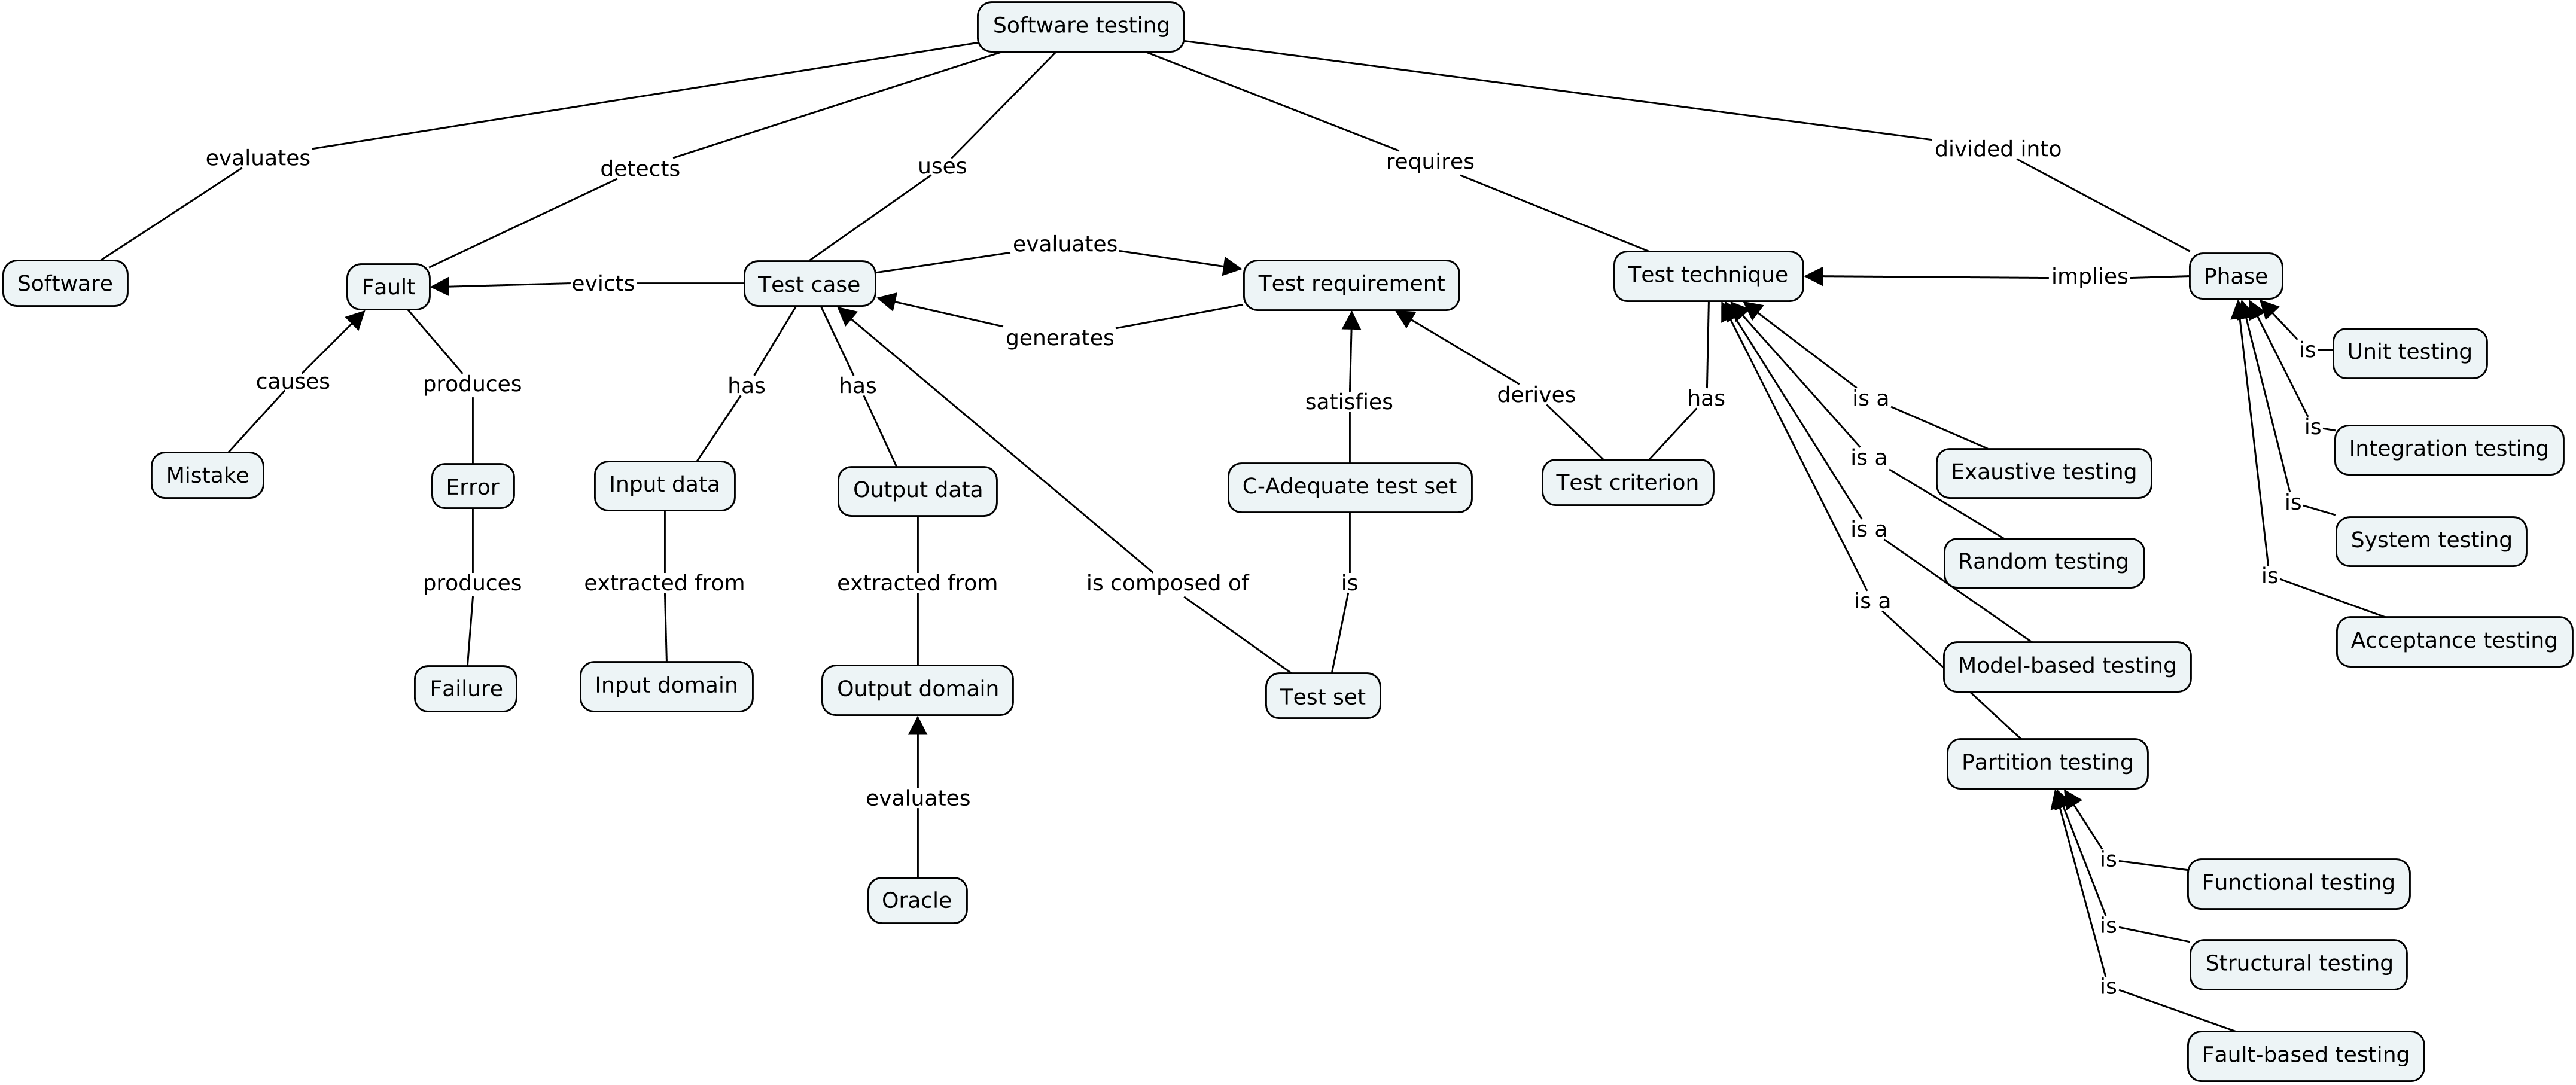
\includegraphics[width=\textwidth]{../BasicConcepts/Software testing fundamentals.png}
\end{frame}



\mainmatter{}
\part{Fault-based testing}
\section{Fault-based testing}
\begin{frame}[hasprev=false, hasnext=true, fragile]
\frametitle{Fault-based testing example}
\label{example:fault-based-testing}

\begin{block}{Example}
Consider the following source code snippet \cite[p. 45]{myers:2004}.
\end{block}

\begin{block}{Source code}
\vspace{-.15cm}
\begin{lstlisting}[language=java]
public void foo(int a, int b, int x) {
	if (a > 1 && b == 0) {
		x = x/a;
	}
	if (a == 2 || x > 1) {
		x = x + 1;
	}
}
\end{lstlisting}
\end{block}
\end{frame}


\begin{frame}[hasprev=true, hasnext=true, fragile]
\frametitle{Fault-based testing}

\begin{block}{Mutation analysis}
\begin{itemize}
	\item Mutation analysis performs single changes in the source code.

	\item For example, comparators such as \srccode{==} can be changed to
	\srccode{!=}.

	\item The following test case will reveal the error in the mutant:
	\begin{itemize}
		\item $a = 3, b = 0, x = 3$
	\end{itemize}
\end{itemize}
\end{block}

\begin{block}{Original application}
\vspace{-.20cm}
\begin{lstlisting}[language=java]
public int foo(int a, int b, int x) {
	if (a > 1 && b == 0) {
		x = x/a;
	}
	if (a == 2 || x > 1) {
		x = x + 1;
	}
	return x;
}
\end{lstlisting}
\end{block}
\end{frame}


\begin{frame}[hasprev=true, hasnext=false, fragile]
\frametitle{Fault-based testing}

\begin{block}{Mutation analysis}
\begin{itemize}
	\item Mutation analysis performs single changes in the source code.

	\item For example, comparators such as \srccode{==} can be changed to
	\srccode{!=}.

	\item The following test case will reveal the error in the mutant:
	\begin{itemize}
		\item $a = 3, b = 0, x = 3$
	\end{itemize}
\end{itemize}
\end{block}

\begin{block}{Mutant}
\vspace{-.20cm}
\begin{lstlisting}[language=java]
public int foo(int a, int b, int x) {
	if (a > 1 && b != 0) {
		x = x/a;
	}
	if (a == 2 || x > 1) {
		x = x + 1;
	}
	return x;
}
\end{lstlisting}
\end{block}

\end{frame}

\subsection{Error seeding}
\include{main/fault-based-testing/error-seeding}

\part{Mutation testing}
\subsection{Mutation testing}
\include{main/fault-based-testing/mutation}

\subsubsection{Mutant}
\include{main/fault-based-testing/mutation/mutant}

\subsubsection{Mutant operator}
\include{main/fault-based-testing/mutation/mutant-operator}

\subsubsection{Mutantion approach}
\include{main/fault-based-testing/mutation/mutation-approach}

\part{References and credits}
\backmatter{}
\include{bibliography}
\part{Acknowledgement}
\section*{Acknowledgement}


\begin{frame}[c,label=credits]
\frametitle{Credits}

\centering
\animategraphics[height=140pt,poster=first,autoplay,loop]{1}{main/jabuti-}{0}{3}

\begin{itemize}
	\item Reviewers:
	\begin{itemize}
		% \item Auri Marcelo Rizzo Vincenzi
		% \item Ellen Francine Barbosa
		\item Fabiano Cutigi Ferrari
		% \item Márcio Eduardo Delamaro
		\item Otávio Augusto Lazzarini Lemos
	\end{itemize}
\end{itemize}
\end{frame}


\part{Instructional elements}
\include{examples}
\include{exercises}

\end{document}
